\documentclass[12pt]{article}
\usepackage{graphicx}
\usepackage{listings}
\usepackage{xcolor}
\usepackage{hyperref}
\definecolor{dkgreen}{rgb}{0,0.6,0}
  \definecolor{gray}{rgb}{0.5,0.5,0.5}
  \definecolor{mauve}{rgb}{0.58,0,0.82}
  \definecolor{greyish}{rgb}{0.96,0.96,0.96}

  \lstset{
    backgroundcolor=\color{greyish},   % choose the background color; you must add \usepackage{color} or \usepackage{xcolor}
    frame=tblr,
    numbers=left,                       % where to put the line-numbers; possible values are (none, left, right)
    numbersep=5pt,                   % how far the line-numbers are from the code
    numberstyle=\tiny\color{mygray}, % the style that is used for the line-numbers
    language=Ruby,
    aboveskip=3mm,
    belowskip=3mm,
    showstringspaces=false,
    columns=flexible,
    basicstyle={\footnotesize\ttfamily},
    numbers=none,
    numberstyle=\tiny\color{gray},
    keywordstyle=\color{blue},
    commentstyle=\color{dkgreen},
    stringstyle=\color{mauve},
    breaklines=true,
    breakatwhitespace=true
    tabsize=1
  }
\begin{document}

\begin{titlepage}
\begin{center} 
 \textsc{\large Facultatea Calculatoare, Informatica si Microelectronica}\\[0.5cm]
\textsc{\large Universitatea Tehnica a Moldovei}\\[1.2cm] 
\vspace{25 mm}

\textsc{\Large Medii Interactive de Dezvoltare a Produselor Soft}\\[0.5cm] 
\textsc{\large Lucrarea de laborator\#5}\\[0.5cm] \newcommand{\HRule}{\rule{\linewidth}{0.5mm}} 
  \vspace{10 mm}
  \HRule \\[0.4cm]
  { \LARGE \bfseries Dezvoltarea unei aplicatii mobile  }\\[0.4cm] 
  \HRule \\[1.5cm]
      \vspace{30mm}

      \begin{minipage}{0.4\textwidth}
      \begin{flushleft} \large
      \emph{Autor:}\\
      Alexandr \textsc{Ialticenco}
      \end{flushleft}
      \end{minipage}
      ~
      \begin{minipage}{0.4\textwidth}
      \begin{flushright} \large
      \emph{lector asistent:} \\
      Irina \textsc{Cojanu} \\ 
      \emph{lector superior:} \\
      Svetlana \textsc{Cojocaru} 
      \end{flushright}
      \end{minipage}\\[4cm]

      \vspace{5 mm}

      \vfill
      \end{center}
      
\end{titlepage}

\section*{Obiectivele lucrarii}
\begin{itemize}
\item Cunostinte de baza privina arhitectura unei aplicatii mobile
\item Cunostinte de baza ale platformei SDK
\end{itemize}

\section* {Sarcina lucrarii}
\textbf{Advanced level:}
\begin{itemize}
\item Realizeaza o aplicatie care va implimenta tehnica Pomodoro SAU
\item O alta aplicatie sofisticata la alegere
Game
\end{itemize}
\section* {Cerinte tehnice}
\begin{itemize}
\item Foloseste un nou IDE pentru fiecare lucrare de laborator
\end{itemize}
\section* {Bonus Point}
\begin{itemize}
\item Folosirea Facebook/Twitter/Google Maps API
\end{itemize}
\section {Configurarea IDE-ului Android Studio}
\subsection{Instalarea}
Android Studio este absolut gratuit si poate fi descarcat de pe pagina oficiala: \url{http://developer.android.com/sdk/}
\newpage 
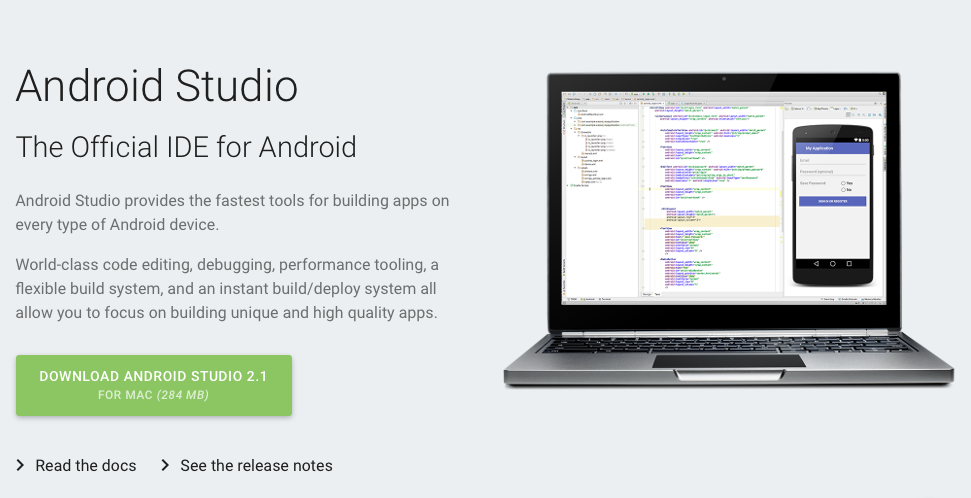
\includegraphics[width=12.5cm]{images/1}
\subsection{Crearea unui proiect}
Pentru a crea un proiect nou trebuie doar de apelat optiunea corespunzatoare din meniul. Android Studio va cere ca sa fie introduse numele de package si alte atribute obligatorii pentru proiect android. \\
\\
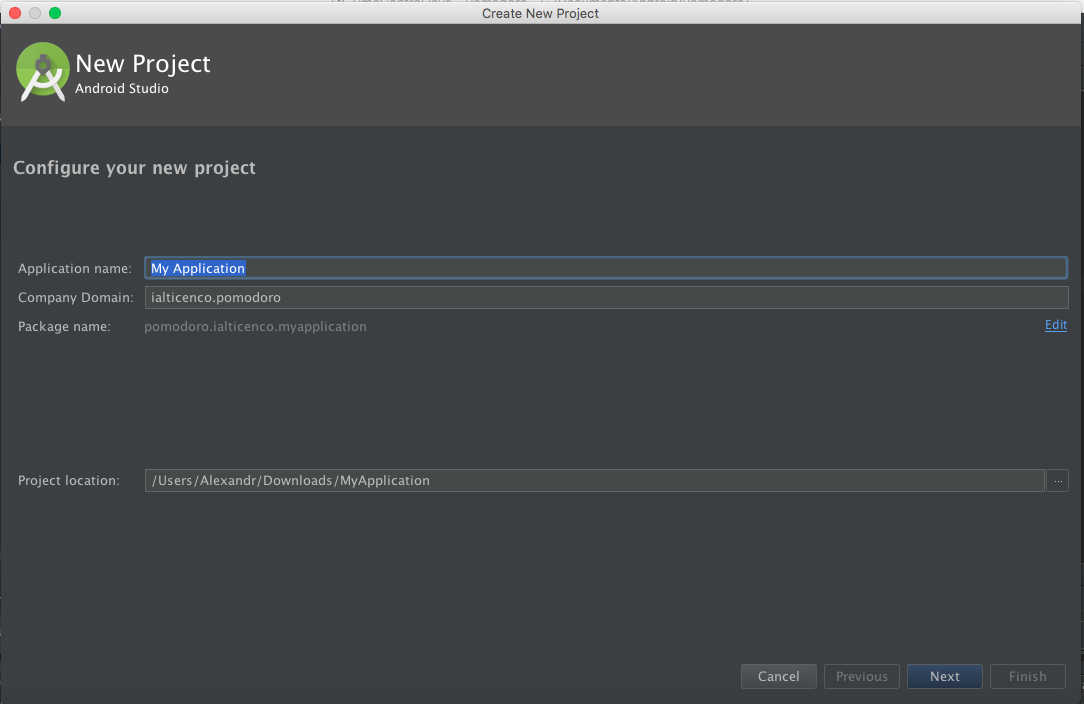
\includegraphics[width=12.5cm]{images/2}
\subsection{Configurarea emulatorului}
Pentru a testa rezultatele lucrarii vom utiliza emulatorul genymotion care ne ofera nu doar posibilitate de a face debug mai rapid si comod decat prin intermediul unui telefon-android real dar si productivitatea mai mare decat emulatorul oferit de catre Google in complect cu Android Studio. \\\\
Emulatorul Genymotion la fel este gratuit pentru scopuri necomerciale si poate fi usor descarcat de pe pagina oficiala.\\\\
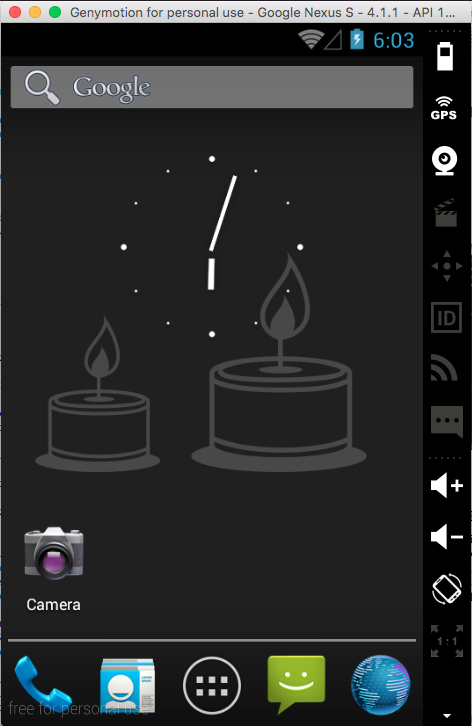
\includegraphics[height=11.5cm]{images/3}\\
\section {Listingul}
\subsection{PomodoroActivity}
Orice aplicatia android consta din diferite acitivity (una principala cu intent filter (MAIN/LAUNCHER) si mai multe altele). Activity reprezinta o cale de afisa datele in aplicatia android prin intermediul android layout (sunt prezente in fisierele /res/layout*.xml ). In aplicatia Pomodoro o sa fie suficienta doar o Activity. Descriem clasa ei in fisierul cu un nume corespunzator.
\begin{lstlisting}[language=java, caption={Fisierul PomodoroActivity.java}, label=list2]
<?php
package ialticenco.pomodoro;

import android.app.Activity;
import android.content.SharedPreferences;
import android.graphics.Bitmap;
import android.graphics.BitmapFactory;
import android.graphics.Color;
import android.media.MediaPlayer;
import android.net.Uri;
import android.os.Handler;
import android.os.Message;
import android.preference.PreferenceManager;
import android.support.v7.app.AppCompatActivity;
import android.os.Bundle;
import android.util.Log;
import android.view.View;
import android.widget.ImageView;

import com.facebook.CallbackManager;
import com.facebook.FacebookCallback;
import com.facebook.FacebookException;
import com.facebook.FacebookSdk;
import com.facebook.share.Sharer;
import com.facebook.share.model.ShareLinkContent;
import com.facebook.share.widget.ShareDialog;

public class PomodoroActivity extends Activity {
    public enum State {WORK, REST, NONE, PAUSE};
    public static State savedState;
    public static State state;
    public static int timer;
    public static int workMax = 1500;
    public static int restMax = 300;
    public static int ultraRestMax = 900;
    public static int timerLimit;
    public static int workPeriod = 0;
    public static View root;
    public static Handler handler;
    public static ImageView playButton, stopButton, settingsButton, facebookButton;
    public static String workLabel = "Working...", restLabel="Relaxing...", noLabel="Press play to start", pauseLabel="Paused..";
    public static MediaPlayer mp;
    public static PomodoroActivity MainScreen;
    CallbackManager callbackManager;
    ShareDialog shareDialog;
    @Override
    protected void onCreate(Bundle savedInstanceState) {
        super.onCreate(savedInstanceState);
        state = State.NONE;
        MainScreen = this;
        TimeControl.noColor = Color.BLUE;
        TimeControl.workColor = Color.parseColor("#850000");
        TimeControl.restColor = Color.parseColor("#0b7000");
        setContentView(R.layout.activity_pomodoro);
        root = findViewById(R.id.root);
        root.setBackgroundColor(TimeControl.noColor);
        initInterface();
        handler = new Handler(new Handler.Callback() {
            @Override
            public boolean handleMessage(Message message) {
                root.setBackgroundColor(TimeControl.currentColor);
                return false;
            }
        });
        load();
        FacebookSdk.sdkInitialize(getApplicationContext());
        callbackManager = CallbackManager.Factory.create();
        shareDialog = new ShareDialog(this);
        shareDialog.registerCallback(callbackManager, new FacebookCallback<Sharer.Result>() {
            @Override
            public void onSuccess(Sharer.Result result) {

            }

            @Override
            public void onCancel() {

            }

            @Override
            public void onError(FacebookException error) {

            }
        });

    }
    public static String convertTime(int time){
        String min = time/60+"";
        String sec = time %60+"";
        if (min.length()<2) min = "0"+min;
        if (sec.length()<2) sec = "0"+sec;
        return min+":"+sec;
    }
    public void initInterface(){
        playButton = (ImageView) findViewById(R.id.play);
        playButton.setOnClickListener(new View.OnClickListener() {
            @Override
            public void onClick(View view) {
                switch(state){
                    case WORK: pause(); break;
                    case REST: pause(); break;
                    case NONE: startWork(); playButton.setImageResource(R.drawable.pause); break;
                    case PAUSE: resume(); break;
                }
            }
        });
        stopButton = (ImageView) findViewById(R.id.stop);
        stopButton.setOnClickListener(new View.OnClickListener() {
            @Override
            public void onClick(View view) {
                state = State.NONE;
                TimeControl.currentLabel = noLabel;
                playButton.setImageResource(R.drawable.play);
                TimeControl.currentColor = TimeControl.noColor;
                root.setBackgroundColor(TimeControl.currentColor);
            }
        });
        settingsButton = (ImageView) findViewById(R.id.settings);
        settingsButton.setOnClickListener(new View.OnClickListener() {
            @Override
            public void onClick(View view) {
                SettingsDialog.showDialog();
            }
        });
        facebookButton = (ImageView) findViewById(R.id.facebook);
        facebookButton.setOnClickListener(new View.OnClickListener() {
            @Override
            public void onClick(View view) {
                if (ShareDialog.canShow(ShareLinkContent.class)) {
                    ShareLinkContent linkContent = new ShareLinkContent.Builder()
                            .setContentTitle("Pomodoro App")
                            .setContentDescription(
                                    "Download right now pomodoro app and change your life!")
                            .setContentUrl(Uri.parse("http://
                            developers.facebook.com/android"))
                            .build();

                    shareDialog.show(linkContent);
                }
            }
        });
    }

    public static void pause(){
        Log.d("STATECHANGE","PAUSE");
        savedState = state;
        state = State.PAUSE;
        TimeControl.currentLabel = pauseLabel;
        playButton.setImageResource(R.drawable.play);
    }

    public static void resume(){
        Log.d("STATECHANGE","RESUME");
        state = savedState;
        playButton.setImageResource(R.drawable.pause);
        switch (state){
            case WORK: TimeControl.currentLabel = workLabel; break;
            case REST: TimeControl.currentLabel = workLabel; break;
        }
    }
    public static void startWork(){
        Log.d("STATECHANGE","WORK");
        timer = 0;
        timerLimit = workMax;
        TimeControl.time = convertTime(timer);
        state = State.WORK;
        TimeControl.currentColor = TimeControl.workColor;
        handler.sendEmptyMessage(0);
        TimeControl.currentLabel = workLabel;
        workPeriod++;
    }
    public static void startRest(){
        Log.d("STATECHANGE","REST");
        timer = 0;
        timerLimit = workPeriod<4?restMax:ultraRestMax;
        if (workPeriod >= 4)
            workPeriod = 0;
        TimeControl.time = convertTime(timer);
        state = State.REST;
        TimeControl.currentColor = TimeControl.restColor;
        TimeControl.currentLabel = restLabel;
        handler.sendEmptyMessage(0);
    }
    public static void playSound(){
        mp = MediaPlayer.create(TimeControl.context, R.raw.ring);
        mp.setOnCompletionListener(new MediaPlayer.OnCompletionListener() {
            @Override
            public void onCompletion(MediaPlayer mp) {
                // TODO Auto-generated method stub
                mp.reset();
                mp.release();
                mp = null;
                mp=null;
            }

        });
        mp.start();
    }

    public void load(){
        SharedPreferences sPref = PreferenceManager.getDefaultSharedPreferences(this);
        workMax = Integer.parseInt(sPref.getString("work", "1500"));
        restMax = Integer.parseInt(sPref.getString("rest", "300"));
        ultraRestMax = Integer.parseInt(sPref.getString("ultra", "900"));
    }
}
\end{lstlisting}
Activity va contine suprafata de afisare timerului (componenta SurfaceView) si patru butoane: Play/Pause, Stop, Settings, Facebook Share. Mai jos este prezenta XML-sursa fisierului android layout utilizat pentru a initializa PomodoroActivity in metoda onCreate.\\\\

\begin{lstlisting}[language=xml, caption={Fisierul activity\_pomodoro.xml}, label=list2]
<?xml version="1.0" encoding="utf-8"?>
<LinearLayout xmlns:android="http://schemas.android.com/apk/res/android"
    xmlns:tools="http://schemas.android.com/tools"
    android:layout_width="match_parent"
    android:layout_height="match_parent"
    android:paddingBottom="@dimen/activity_vertical_margin"
    android:paddingLeft="@dimen/activity_horizontal_margin"
    android:paddingRight="@dimen/activity_horizontal_margin"
    android:paddingTop="@dimen/activity_vertical_margin"
    tools:context="ialticenco.pomodoro.PomodoroActivity"
    android:orientation="vertical"
    android:background="#ff0000"
    android:id="@+id/root">

    <ialticenco.pomodoro.TimeControl
        android:layout_width="match_parent"
        android:layout_height="0dp"
        android:id="@+id/surfaceView"
        android:layout_centerVertical="true"
        android:layout_centerHorizontal="true"
        android:layout_weight="3.5"
        android:background="#ff0000" />

    <RelativeLayout
        android:layout_width="match_parent"
        android:layout_height="0dp"
        android:layout_gravity="center_horizontal"
        android:layout_weight="1">

        <LinearLayout
            android:orientation="horizontal"
            android:layout_width="wrap_content"
            android:layout_height="wrap_content"
            android:layout_centerInParent="true">

            <ImageView
                android:layout_width="48dp"
                android:layout_height="48dp"
                android:id="@+id/play"
                android:layout_margin="10dp"
                android:src="@drawable/play" />

            <ImageView
                android:layout_width="48dp"
                android:layout_height="48dp"
                android:id="@+id/stop"
                android:layout_margin="10dp"
                android:src="@drawable/stop" />

            <ImageView
                android:layout_width="48dp"
                android:layout_height="48dp"
                android:id="@+id/settings"
                android:layout_margin="10dp"
                android:src="@drawable/settings" />

            <ImageView
                android:layout_width="48dp"
                android:layout_height="48dp"
                android:id="@+id/facebook"
                android:layout_margin="10dp"
                android:src="@drawable/facebook" />
        </LinearLayout>
    </RelativeLayout>

</LinearLayout>
\end{lstlisting}
Pentru a implementa butoanele vom utiliza componenta ImageView care ne va oferi posibilitate de a schimba usor si simplu background-ul (imagina butonului vazuta de utilizator). \newpage
\subsection{Afisarea graficii}
Pentru a afisa cronometrul vom utiliza SurfaceView si respectiv canvas-ul lui. Pentru a ridica productivitatea vom desena intr-un alt thread (inner clasa DrawThread encapsuleaza metodele de apelare la canvas. 
\begin{lstlisting}[language=java, caption={Fisierul TimeControl.java}, label=list2]
package ialticenco.pomodoro;

import android.content.Context;
import android.graphics.Bitmap;
import android.graphics.BitmapFactory;
import android.graphics.Canvas;
import android.graphics.Color;
import android.graphics.Matrix;
import android.graphics.Paint;
import android.graphics.Path;
import android.graphics.RectF;
import android.graphics.Typeface;
import android.util.AttributeSet;
import android.util.Log;
import android.view.SurfaceHolder;
import android.view.SurfaceView;

/**
 * Created by Alexandr on 25.04.16.
 */
public class TimeControl extends SurfaceView implements SurfaceHolder.Callback{
    public static TimeControl engine;
    public static Context context;
    public static int Width, Height;
    public static float Proportion;
    public static DrawThread drawThread;
    public static Paint paint, paint2;
    public static Path path;
    public static int noColor, workColor, restColor;
    public static int currentColor;
    public static float progress = 0.5f;
    public static RectF rect;
    public static String time;
    public static Typeface font;
    public static Typeface defaultFont;
    public static long prev;
    public static String currentLabel;
    public static Bitmap pomodora, little;
    public static float koef = 1f, inc = 0.01f;
    public static boolean growing;

    public TimeControl(Context context){
        super(context);
        engine = this;
        this.context = context;
        getHolder().addCallback(this);
        currentColor = noColor;
    }
    public TimeControl(Context context, AttributeSet attrs){
        super(context);
        if (pomodora == null)
            pomodora = BitmapFactory.decodeResource(context.getResources(),
                    R.drawable.logo);
        if (little == null)
            little = BitmapFactory.decodeResource(context.getResources(),
                    R.drawable.little);
        engine = this;
        this.context = context;
        getHolder().addCallback(this);
        currentColor = noColor;
        font= Typeface.createFromAsset(context.getAssets(),"alarm.ttf");
        defaultFont= Typeface.createFromAsset(context.getAssets(),"arial.ttf");
        currentLabel = PomodoroActivity.noLabel;
    }
    @Override
    public void surfaceCreated(SurfaceHolder surfaceHolder) {
        Log.d("DRAWT","CREATED");
        paint = new Paint();
        paint2 = new Paint();
        paint.setTypeface(font);
        paint2.setTypeface(defaultFont);
        drawThread = new DrawThread(this.getHolder());
        drawThread.setRunning(true);
        drawThread.start();
        prev = System.currentTimeMillis();
    }

    @Override
    public void surfaceChanged(SurfaceHolder surfaceHolder, int i, int i1, int i2) {

    }

    @Override
    public void surfaceDestroyed(SurfaceHolder surfaceHolder) {
        drawThread.setRunning(false);
    }

    class DrawThread extends Thread {

        private boolean running = false;
        private SurfaceHolder surfaceHolder;

        public DrawThread(SurfaceHolder surfaceHolder) {
            this.surfaceHolder = surfaceHolder;
        }

        public void setRunning(boolean running) {
            this.running = running;
        }

        @Override
        public void run() {
            while(running){
                Canvas canvas = null;
                try {
                    canvas = surfaceHolder.lockCanvas(null);
                    if (PomodoroActivity.state != PomodoroActivity.State.NONE &&  PomodoroActivity.state != PomodoroActivity.State.PAUSE) {
                        if (System.currentTimeMillis() - prev >= 1000){
                            prev = System.currentTimeMillis();
                            if (PomodoroActivity.timer < 
                            PomodoroActivity.timerLimit)
                                PomodoroActivity.timer += 60;
                            else {
                                switch (PomodoroActivity.state){
                                    case WORK:  PomodoroActivity.playSound(); PomodoroActivity.startRest(); break;
                                    case REST: PomodoroActivity.playSound(); PomodoroActivity.startWork(); break;
                                }
                            }
                        }
                    }
                    if (canvas == null)
                        continue;
                    Width = canvas.getWidth();
                    Height = canvas.getHeight();
                    Proportion = Height/768.0f;
                    drawTime(canvas);
                    //Log.d("DRAWT","DRAWING");

                } finally {
                    if (canvas != null) {
                        surfaceHolder.unlockCanvasAndPost(canvas);
                        postInvalidate();
                    }
                }
            }
        }

    }
    public void drawImage(Canvas canvas,Bitmap bmp, float left, float top,float width, float height, Paint paint){
        left *= Width;
        top *= Height;
        width *= Width;
        height *= Height;
        Matrix matrix = new Matrix();
        matrix.reset();
        matrix.setTranslate(left, top);
        matrix.preScale(width / bmp.getWidth(), height / bmp.getHeight());
        canvas.drawBitmap(bmp, matrix, paint);
    }

    public void drawImageCenter(Canvas canvas, Bitmap bmp, float x, float y, float w, float h, Paint paint){
        x *= Width;
        y *= Height;
        w *= Width;
        h *= Height;
        Matrix matrix = new Matrix();
        matrix.reset();
        matrix.setTranslate(x - w / 2, y - h / 2);
        matrix.preScale(w / bmp.getWidth(), h / bmp.getHeight());
        canvas.drawBitmap(bmp, matrix, paint);
    }

    public static int getX(float x){
        return (int)(x*Width);
    }
    public static int getY(float y){
        return (int)(y*Height);
    }
    public static int getM(float m){
        return (int)(m*((Height+Width)/2));
    }
    public static int getCenterX(){
        return Width/2;
    }
    public static int getCenterY(){
        return Height/2;
    }
    public static int fromCenterX(float x){
        return getCenterX()+(int)(x*Width);
    }
    public static int fromCenterY(float y){
        return getCenterY()+(int)(y*Width);
    }
    public void drawTime(Canvas canvas){
        switch (PomodoroActivity.state){
            case NONE: inc = 0.01f; break;
            case PAUSE: inc = 0f; break;
            default: inc = 0.02f; break;
        }
        /*if (progress<1f)
            progress += 0.00f;
        else progress = 1f;*/
        if (growing){
            if (koef<1.5f)
                koef += inc;
            else
                growing = false;
        } else {
            if (koef>1.0f)
                koef -= inc;
            else
                growing = true;
        }
        time = System.currentTimeMillis()/1000+"";
        progress = (1f*PomodoroActivity.timer)/PomodoroActivity.timerLimit;
        canvas.drawColor(currentColor);
        if (PomodoroActivity.state == PomodoroActivity.State.NONE)
        drawImageCenter(canvas, pomodora,0.5f,0.5f,0.5f*koef,0.3f*koef,paint);
        else {
            if (PomodoroActivity.state != PomodoroActivity.State.PAUSE)
                drawImageCenter(canvas, little,0.5f,0.425f,0.25f*koef,0.18f*koef,paint);
            else
                drawImageCenter(canvas, little,0.5f,0.425f,0.25f*koef,0.18f*koef,paint);
        }
        paint.setColor(Color.WHITE);
        if (path == null) {
            path = new Path();
            rect = new RectF(fromCenterX(-0.35f), fromCenterY(-0.45f), fromCenterX(0.35f), fromCenterY(0.25f));
            path.addArc(rect, 0, 360);
        }
        paint.setStrokeWidth(32*Proportion);
        paint.setStyle(Paint.Style.STROKE);
        if (PomodoroActivity.state != PomodoroActivity.State.NONE)
        canvas.drawPath(path, paint);
        paint.setColor(currentColor);
        paint.setStrokeWidth(16*Proportion);
        Path path2 = new Path();
        if (PomodoroActivity.state != PomodoroActivity.State.NONE)
        path2.addArc(rect,0,360*progress);
        else
            path2.addArc(rect,0,360);
        if (PomodoroActivity.state != PomodoroActivity.State.NONE)
        canvas.drawPath(path2, paint);
        paint.setStrokeWidth(2);
        paint.setTextAlign(Paint.Align.CENTER);
        paint.setColor(Color.WHITE);
        paint.setTextSize(64*Proportion);
        time = PomodoroActivity.convertTime(PomodoroActivity.timer);
        if (PomodoroActivity.state != PomodoroActivity.State.NONE)
        canvas.drawText(time,getCenterX(),getCenterY() + getY(-0.05f*Proportion),
         paint);
        paint2.setColor(Color.WHITE);
        paint2.setTextSize(64*Proportion);
        paint2.setTextAlign(Paint.Align.CENTER);
        canvas.drawText(currentLabel,getCenterX(), 
        getCenterY()+getY(0.5f*Proportion),paint2);
    }
}
\end{lstlisting}
Metoda drawTime() este responsabila pentru redesenarea fiecarui nou frame, afisarea timerului si textului. Metodele drawImage si drawImageCenter ajuta sa faca un cod sursa mai clar si eficient. Pentru a realiza partea grafica a aplicatiei am ales sa utilizam sistemul de coordinate de la 0 pana la 1. Lucrul acesta ne-a oferit posibilitate sa nu pierdem proportii de imagini afisate independent de rezolutia ecranului device-ului pe care sa fie instalata aplicatia noastra. Metodele getX, getY, getCenterX, getCenterY proceseaza coordonatele oferite de catre programator in unitatile decemale si le transforma intr-un limbal de pixel.
\subsection{Settings Dialog}
Pentru a oferi utilizatorului nostru posibilitatea de a modifica durata perioadelor de lucru si de odihna am introdus un dialog special, care contine trei TextView, trei EditText si doua butoane standarte - Save si Cancel. In codul sursa a clasei SettingsDialog sunt descrise afisarea dialogului si modul in care aplicatia proceseaza actiunile utilizatorului asupra campurilor de text si butoanelor. Metoda save contine o secventa de comande care salveaza noile setari in SharedPrefferences (aceasta cale de stocare a configurarilor este propusa programatorilor de catre Google). Clasa PomodoroActivity descrisa mai sus contine inca o clasa legata de SharedPrefferences. Ea citeste setarile stocate si le aplica inainte de a afisa interfata utilizatorului.
\begin{lstlisting}[language=php, caption={Fisierul SettingsDialog.php}, label=list2]
package ialticenco.pomodoro;

/**
 * Created by Alexandr on 27.04.16.
 */

import android.app.Dialog;
import android.content.Context;
import android.content.SharedPreferences;
import android.graphics.Color;
import android.graphics.drawable.ColorDrawable;
import android.graphics.drawable.GradientDrawable;
import android.os.Bundle;
import android.preference.PreferenceManager;
import android.view.MotionEvent;
import android.view.View;
import android.view.Window;
import android.widget.Button;
import android.widget.EditText;
import android.widget.TextView;

/**
 * Created by Alexandr on 27.12.15.
 */
public class SettingsDialog extends Dialog implements View.OnClickListener, View.OnTouchListener{
    private Button yes, no;
    private static int gift;
    public static boolean isClosing = true;
    public EditText worktime, resttime, ultraresttime;
    public Button saveButton, cancelButton;

    public SettingsDialog(Context context) {
        super(context);
    }
    @Override
    protected void onCreate(Bundle savedInstanceState) {
        super.onCreate(savedInstanceState);
        requestWindowFeature(Window.FEATURE_NO_TITLE);
        setContentView(R.layout.settings_dialog);
        worktime = (EditText)findViewById(R.id.worktime);
        resttime = (EditText)findViewById(R.id.resttime);
        ultraresttime = (EditText)findViewById(R.id.ultraresttime);
        worktime.setText((PomodoroActivity.workMax/60)+"");
        resttime.setText((PomodoroActivity.restMax/60)+"");
        ultraresttime.setText((PomodoroActivity.ultraRestMax/60)+"");
        worktime.setSelection(worktime.getText().length());
        resttime.setSelection(resttime.getText().length());
        ultraresttime.setSelection(ultraresttime.getText().length());
        saveButton = (Button)findViewById(R.id.saveButton);
        cancelButton = (Button)findViewById(R.id.cancelButton);
        saveButton.setOnClickListener(new View.OnClickListener() {
            @Override
            public void onClick(View view) {
                int work = 25;
                try{
                    work = Integer.parseInt(worktime.getText().toString());
                } catch (Exception e){

                }
                if (work<1) work = 1; else
                if (work>1000) work = 1000;
                int rest = 5;
                try{
                    rest = Integer.parseInt(resttime.getText().toString());
                } catch (Exception e){

                }
                if (rest<1) rest = 5; else
                if (rest>1000) rest = 1000;
                int ultra = 25;
                try{
                    ultra = Integer.parseInt(worktime.getText().toString());
                } catch (Exception e){

                }
                if (ultra<1) ultra = 1; else
                if (ultra>1000) ultra = 1000;
                PomodoroActivity.workMax = work*60;
                PomodoroActivity.restMax = rest*60;
                PomodoroActivity.ultraRestMax = ultra*60;
                save(work*60, rest*60, ultra*60);
                dismiss();
            }
        });
        cancelButton.setOnClickListener(new View.OnClickListener() {
            @Override
            public void onClick(View view) {
                dismiss();
            }
        });
    }


    @Override
    public void onClick(View view) {
        dismiss();
    }
    public static void showDialog(){
        SettingsDialog giftDialog=new SettingsDialog(PomodoroActivity.MainScreen);
        giftDialog.getWindow().setBackgroundDrawable(new ColorDrawable(android.graphics.Color.TRANSPARENT));
        giftDialog.show();

    }

    @Override
    public boolean onTouch(View view, MotionEvent motionEvent) {
        int action = motionEvent.getAction();
        return false;
    }

    public void save(int work, int rest, int ultra){
        SharedPreferences sPref = PreferenceManager.getDefaultSharedPreferences(getContext());
        SharedPreferences.Editor ed = sPref.edit();
        ed.putString("work", work+"");
        ed.putString("rest", rest+"");
        ed.putString("ultra", ultra+"");
        ed.commit();
    }
}

\end{lstlisting}
La fel ca si activity, dialog-ul nu poate fi afisat fara layout care se descrie prin intermediul fisierilor layout de tip XML. Mai jos este prezent settings\_dialog.
\begin{lstlisting}[language=java, caption={Fisierul settings\_dialog.xml}, label=list2]
/package ialticenco.pomodoro;

/**
 * Created by Alexandr on 27.04.16.
 */

import android.app.Dialog;
import android.content.Context;
import android.content.SharedPreferences;
import android.graphics.Color;
import android.graphics.drawable.ColorDrawable;
import android.graphics.drawable.GradientDrawable;
import android.os.Bundle;
import android.preference.PreferenceManager;
import android.view.MotionEvent;
import android.view.View;
import android.view.Window;
import android.widget.Button;
import android.widget.EditText;
import android.widget.TextView;

/**
 * Created by Alexandr on 27.12.15.
 */
public class SettingsDialog extends Dialog implements View.OnClickListener, View.OnTouchListener{
    private Button yes, no;
    private static int gift;
    public static boolean isClosing = true;
    public EditText worktime, resttime, ultraresttime;
    public Button saveButton, cancelButton;

    public SettingsDialog(Context context) {
        super(context);
    }
    @Override
    protected void onCreate(Bundle savedInstanceState) {
        super.onCreate(savedInstanceState);
        requestWindowFeature(Window.FEATURE_NO_TITLE);
        setContentView(R.layout.settings_dialog);
        worktime = (EditText)findViewById(R.id.worktime);
        resttime = (EditText)findViewById(R.id.resttime);
        ultraresttime = (EditText)findViewById(R.id.ultraresttime);
        worktime.setText((PomodoroActivity.workMax/60)+"");
        resttime.setText((PomodoroActivity.restMax/60)+"");
        ultraresttime.setText((PomodoroActivity.ultraRestMax/60)+"");
        worktime.setSelection(worktime.getText().length());
        resttime.setSelection(resttime.getText().length());
        ultraresttime.setSelection(ultraresttime.getText().length());
        saveButton = (Button)findViewById(R.id.saveButton);
        cancelButton = (Button)findViewById(R.id.cancelButton);
        saveButton.setOnClickListener(new View.OnClickListener() {
            @Override
            public void onClick(View view) {
                int work = 25;
                try{
                    work = Integer.parseInt(worktime.getText().toString());
                } catch (Exception e){

                }
                if (work<1) work = 1; else
                if (work>1000) work = 1000;
                int rest = 5;
                try{
                    rest = Integer.parseInt(resttime.getText().toString());
                } catch (Exception e){

                }
                if (rest<1) rest = 5; else
                if (rest>1000) rest = 1000;
                int ultra = 25;
                try{
                    ultra = Integer.parseInt(worktime.getText().toString());
                } catch (Exception e){

                }
                if (ultra<1) ultra = 1; else
                if (ultra>1000) ultra = 1000;
                PomodoroActivity.workMax = work*60;
                PomodoroActivity.restMax = rest*60;
                PomodoroActivity.ultraRestMax = ultra*60;
                save(work*60, rest*60, ultra*60);
                dismiss();
            }
        });
        cancelButton.setOnClickListener(new View.OnClickListener() {
            @Override
            public void onClick(View view) {
                dismiss();
            }
        });
    }


    @Override
    public void onClick(View view) {
        dismiss();
    }
    public static void showDialog(){
        SettingsDialog giftDialog=new SettingsDialog(PomodoroActivity.MainScreen);
        giftDialog.getWindow().setBackgroundDrawable(new ColorDrawable(android.graphics.Color.TRANSPARENT));
        giftDialog.show();

    }

    @Override
    public boolean onTouch(View view, MotionEvent motionEvent) {
        int action = motionEvent.getAction();
        return false;
    }

    public void save(int work, int rest, int ultra){
        SharedPreferences sPref = PreferenceManager.getDefaultSharedPreferences(getContext());
        SharedPreferences.Editor ed = sPref.edit();
        ed.putString("work", work+"");
        ed.putString("rest", rest+"");
        ed.putString("ultra", ultra+"");
        ed.commit();
    }
}


\end{lstlisting}
Pentru a preveni aplicarea setarilor extreme am facut niste verificari, astfel incat timpul indicat in minute poate fi doar in intervalul de la 1 pana la 1000 de minute. Aplicatia verifica datele introduse si le corecteaza in cazul depasirii acestei limite.
\section {Bonus Point: Integrarea si utilizarea Facebook SDK}
Este absolut imposibil de a realiza un proiect serios de succes in domeniul aplicatiilor mobile fara nici o interactiune cu retelele de socializare. In cazul lucrarii de laborator vom inregistra in Facebook for Developers Platform si vom seta aplicatia noastra in asa mod ca sa putem beneficia Facebook API.\\\\
Dupa inregistrare noi am premit Facebook ID pentru aplicatia noastra care trebuie sa fie stocat in /values/strings.xml.  \\
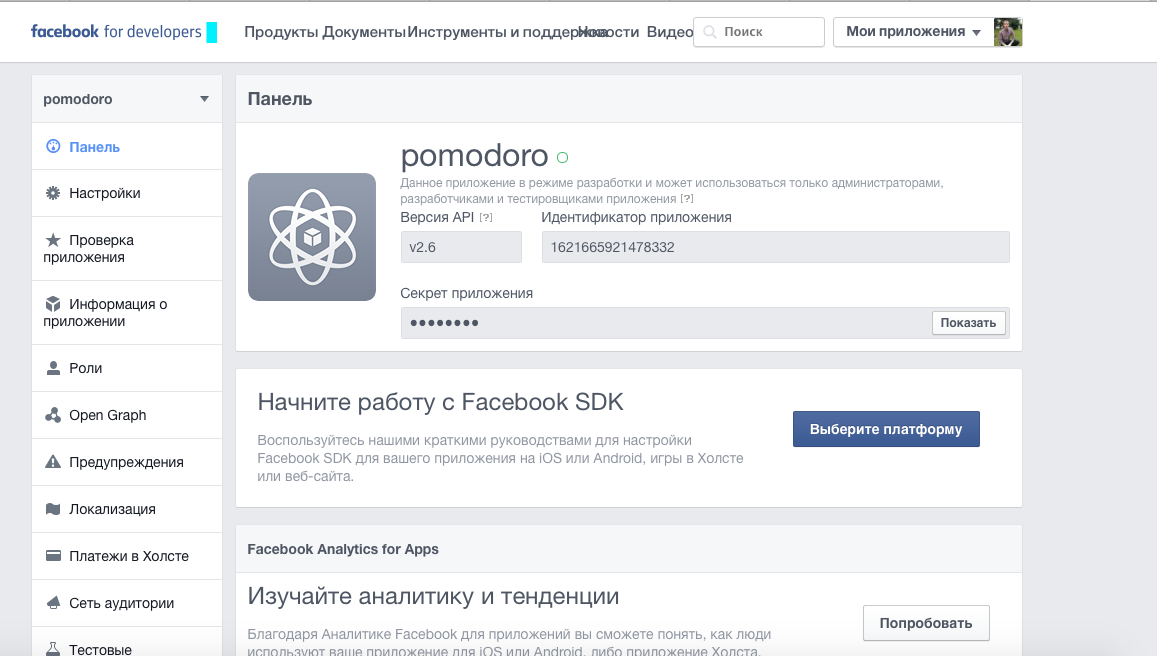
\includegraphics[width=12.5cm]{images/4}\\
Mai mult decat atat am generat si am introdus intr-o forma speciala key hash-ul special care corespunde keystore-ului cu care noi semnam aplicatia.\\\\
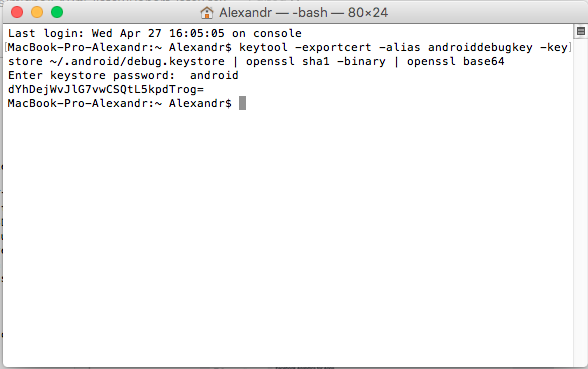
\includegraphics[width=12.5cm]{images/5}\\\\
Dupa editarea AndroidManifest si build.gradle am primit acces la Facebook Android API de la aplicatia noastra. Avand ca un scrop de a realiza ceva simplu am adaugat la aplicatia noastra Share Option ca orice utilizator sa poata sa impartaseasca cu prietenii sai de pe Facebook informatia ca el utilizeaza aplicatia noastra si a obtinut anumite succese.
\\ Lucrul acesta a fost implementat prin intermediul ShareDialog (deja descris in PomodoroActivity.java). Noi doar am legat apasarea butonului coerent cu afisarea dialogului special oferit de Facebook SDK.
\begin{lstlisting}[language=html, caption={Afisarea Facebook Share Dialog}, label=list2]
if (ShareDialog.canShow(ShareLinkContent.class)) {
                    ShareLinkContent linkContent = new ShareLinkContent.Builder()
                            .setContentTitle("Pomodoro App")
                            .setContentDescription(
                                    "Download right now pomodoro app and change your life!")
                            .setContentUrl(Uri.parse("http://
                            developers.facebook.com/android"))
                            .build();

                    shareDialog.show(linkContent);
                }\end{lstlisting}
\section {Rezultatele}
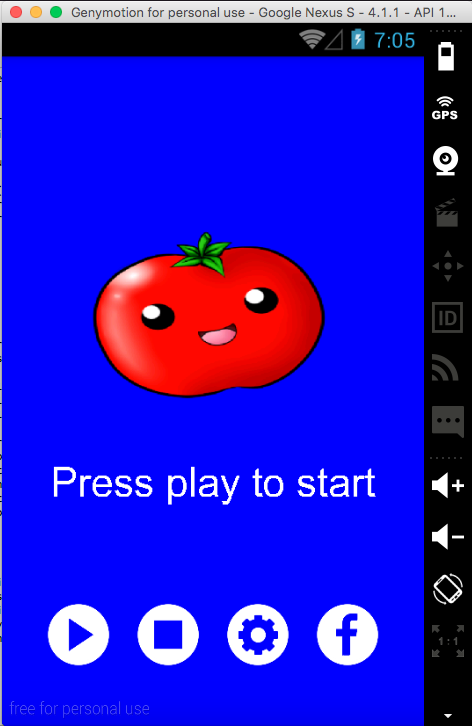
\includegraphics[height=12.5cm]{images/6}
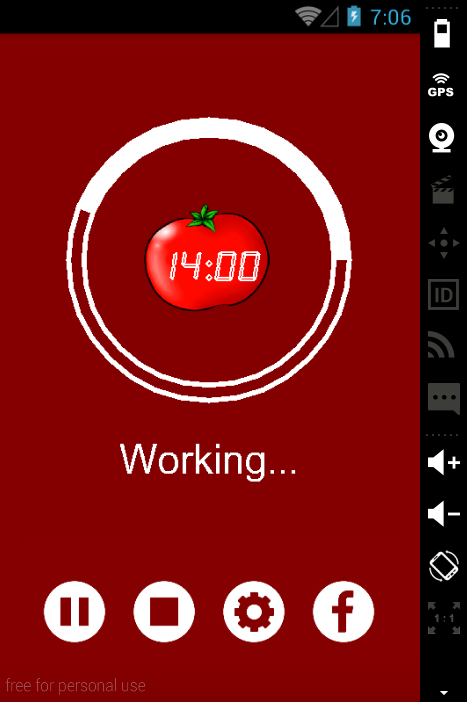
\includegraphics[height=12.5cm]{images/7}\\
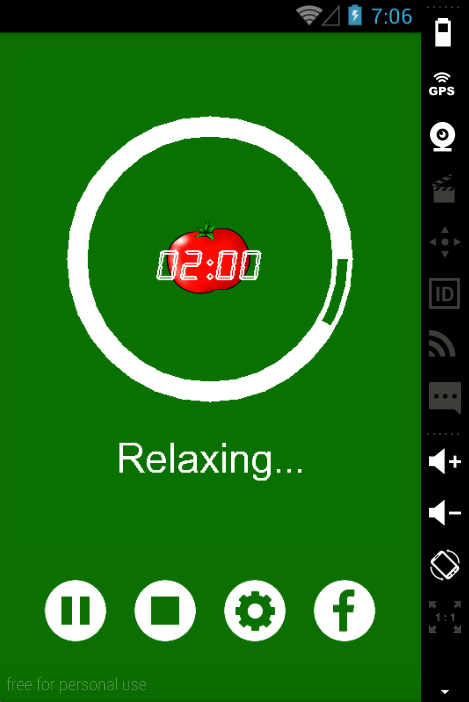
\includegraphics[height=12.5cm]{images/8}
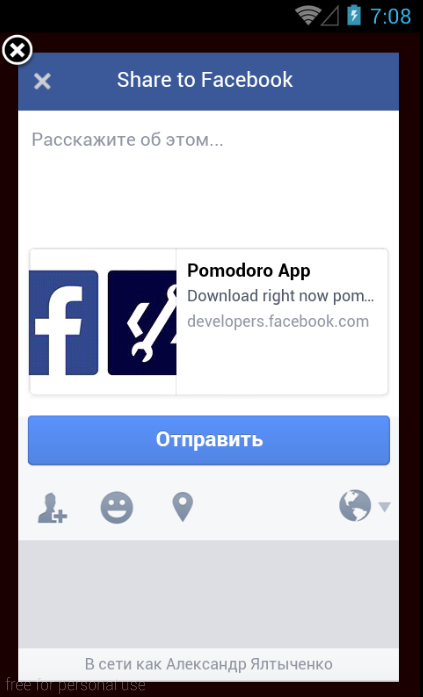
\includegraphics[height=12.5cm]{images/9}
\section*{Concluzii}
In cadrul acestei lucrari de laborator am creat simpla aplicatie mobila care implementeaza tehnica Pomodoro si ofera acces utilizatorului la Facebook API (ca el sa faca niste posturi din numele sau pe pagina sa de facebook fara de a iesi din aplicatia noastra)  prin intermediul IDE-ului Android Studio. Pentru a atinge acest scop am configurat IDE-ul, am instalat si am setat un emulator android pefromant Genymotion si am citit documentatia speciala oferita de catre Google.  Cunostintele obtinute pe parcursul desfasurarii lucrarii de laborator vor fi utile pentru realizarea proiectelor ce urmeaza.
\newpage
\section*{Bibliografie}
\begin{enumerate}
\item http://developer.android.com/guide/index.html - \textbf{Official Android Documentation}
\item https://developers.facebook.com/docs/android/getting-started - \textbf{Official Facebook API Documentation}
\end{enumerate}





\end{document}